% Worked example of one auction with pooled lane bids (analyze/auction_schematic_pooled.py).
\begin{figure}[H]
    \centering
    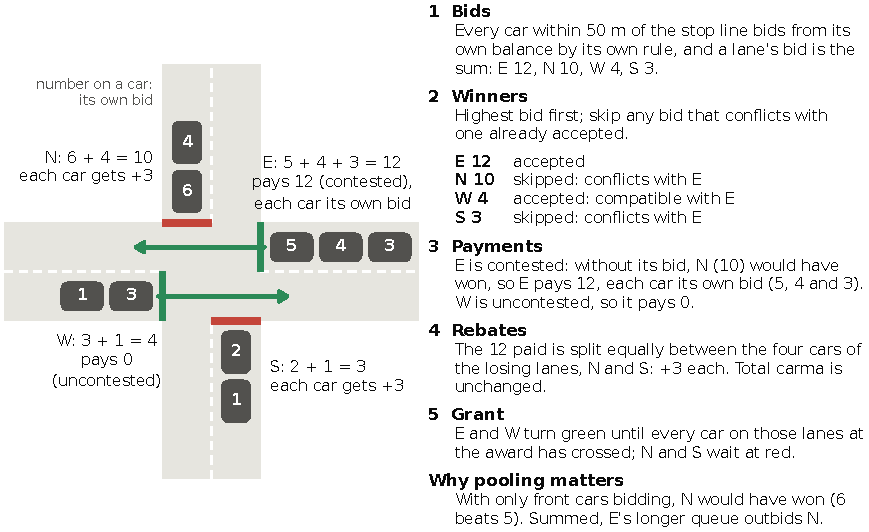
\includegraphics[width=\linewidth]{auction_schematic_pooled.pdf}
    \caption{The auction of Figure~\ref{fig:auction_schematic} with pooled lane bids: every car
    within 50\,m bids from its own balance by its own rule (number on each car) and a lane's bid
    is the sum. The greedy rule (eq.~\eqref{eq:greedy}) accepts E, then W; E is contested and
    pays its total, each car its own bid; W is uncontested and pays nothing; and the 12 paid is
    shared equally among all four cars of the losing lanes. With only front cars bidding, N would
    have won (6 beats 5); pooled, the longer queue on E outbids it. Stop lines show the signal
    after the auction: green for E and W, red for N and S.}
    \label{fig:auction_schematic_pooled}
\end{figure}
